\documentclass[zavrsnirad]{fer}
% Dodaj opciju upload za generiranje konačne verzije koja se učitava na FERWeb
% Add the option upload to generate the final version which is uploaded to FERWeb


\usepackage{blindtext}
\usepackage{bm}
\usepackage{listings}
\usepackage{caption}

\definecolor{codegreen}{rgb}{0,0.6,0}
\definecolor{codegray}{rgb}{0.5,0.5,0.5}
\definecolor{codepurple}{rgb}{0.58,0,0.82}
\definecolor{backcolour}{rgb}{0.95,0.95,0.92}
\lstdefinestyle{mystyle}{
    backgroundcolor=\color{backcolour},
    commentstyle=\color{codegreen},
    keywordstyle=\color{magenta},
    numberstyle=\tiny\color{codegray},
    stringstyle=\color{codepurple},
    basicstyle=\ttfamily\footnotesize,
    breakatwhitespace=false,
    breaklines=true,
    captionpos=t,
    keepspaces=true,
    numbers=left,
    numbersep=5pt,
    showspaces=false,
    showstringspaces=false,
    showtabs=false,
    tabsize=2
}
\lstset{style=mystyle}

\renewcommand*{\lstlistingname}{Izvorni kod}


%--- PODACI O RADU / THESIS INFORMATION ----------------------------------------

% Naslov na engleskom jeziku / Title in English
\title{Multiscale Finite Element Method for heat flow simulations in composites}

% Naslov na hrvatskom jeziku / Title in Croatian
\naslov{Višeskalna metoda konačnih elemenata za simuliranje širenja toplinske energije u kompozitnim materijalima}

% Broj rada / Thesis number
\brojrada{1365}

% Autor / Author
\author{Marko Šelendić}

% Mentor 
\mentor{Izv.\ prof.\ dr.\ sc.\ Dario Bojanjac}

% Datum rada na engleskom jeziku / Date in English
\date{June, 2024}

% Datum rada na hrvatskom jeziku / Date in Croatian
\datum{lipanj, 2024.}

%-------------------------------------------------------------------------------


\begin{document}


% Naslovnica se automatski generira / Titlepage is automatically generated
%\maketitle


%--- ZADATAK / THESIS ASSIGNMENT -----------------------------------------------

% Zadatak se ubacuje iz vanjske datoteke / Thesis assignment is included from external file
% Upiši ime PDF datoteke preuzete s FERWeb-a / Enter the filename of the PDF downloaded from FERWeb
%\zadatak{hr_0036540495_73.pdf}


%--- ZAHVALE / ACKNOWLEDGMENT --------------------------------------------------

\begin{zahvale}
  % Ovdje upišite zahvale / Write in the acknowledgment
  Hvala mojem divnom mentoru Dariju na svoj pomoći i podršci tijekom izrade ovog rada.
\end{zahvale}


% Odovud započinje numeriranje stranica / Page numbering starts from here
\mainmatter


% Sadržaj se automatski generira / Table of contents is automatically generated
\tableofcontents


%--- UVOD / INTRODUCTION -------------------------------------------------------
\chapter{Uvod}\label{pog:uvod}

Kada govorimo o metodama konačnih elemenata, govorimo o nekoliko stvari:
\begin{itemize}
  \item diskretizacija domene (meshiranje)
  \begin{itemize}
    \item rastav na jednostavne konačne elemente poput trokuta, kvadrata, tetraedara, heksaedara, ...
  \end{itemize}
  \item izbor baznih funkcija
  \item definiranje problema u obliku jednadžbe i rubnog uvjeta (ili više njih)
  \begin{itemize}
    \item Poissonova jednadžba, toplinska jednadžba, \ldots
    \item Dirichletovi rubni uvjeti, Neumannovi rubni uvjeti, \ldots
  \end{itemize}
  \item rješavanje problema
\end{itemize}

Razni problemi na koje nailazimo u svijetu i koji zahtijevaju rješavanje pomoću metoda konačnih elemenata,
često uključuju heterogene materijale, odnosno kompozite koji se sastoje od više različitih materijala.
Budući da jedan element naše diskretne domene (eng.\ \textit{mesh}) može biti sastavljen od najviše jednog materijala,
tj.\ može mu biti mapirana samo jedna vrijednost istog svojstva, ovakav pristup zahtijeva diskretizaciju domene
barem onoliko gustu koliko je gusta skala materijala koji se koriste u kompozitu.
Nije teško vidjeti kako ovo može rezultirati velikim brojem elemenata, odnosno velikom numeričkom složenošću i stoga računalnim opterećenjem.

Tradicionalni načini sukobljavanja s ovim problemom uključuju pojednostavljenje svojstava heterogenih materijala,
gdje se ona zamjenjuju homogenom aproksimacijom istog svojstva. Na ovaj način svojstva s fine skale (eng.\ \textit{fine scale}) premjestili smo na
grubu skalu (eng.\ \textit{coarse scale}) te se time riješili potrebe za finom diskretizacijom. Međutim, uvijek kada aproksimiramo,
gubimo dio informacija i točnosti, što u velikom broju slučajeva na kraju ipak ispadne neprihvatljivo.

Višeskalne metode konačnih elemenata (MsFEM) razvijene su kako bi riješile manjkavosti tradicionalnih metoda homogenizacije.
Umjesto aproksimativnog premještanja problema na grubu skalu, ove metode uključuju vršenje aproksimacije svojstva na finoj skali,
i tek onda premještanje i riješavanje problema efikasno na gruboj skali. Jedan od načina na koji to mogu postići jest korištenjem nestandardnih baznih funkcija.
Bazne funkcije bit će konstruirane tako da (aproksimativno) odražavaju heterogena svojstva fine skale, a koristit će se pri rješavanju problema na gruboj skali.

Međutim, u ovom radu fokusirat ćemo se na metodu lokalne ortogonalne dekompozicije (LOD),
koja se osniva na ortogonalnoj podjeli prostora ukupnog rješenja na direktnu sumuprostora rješenja grube i fine skale.
Ova metoda koristi bazne funkcije koje su ortogonalne na prostoru grube skale, te se koriste za rješavanje problema na finoj skali.
Razvit ćemo implementaciju LOD metode za rješavanje višeskalnih problema s prostorno visoko varirajućim koeficijentima toplinske vodljivosti
(ili nekog drugog svojstva) u kompozitnim materijalima. Za definiranje takvih koeficijentata koristit ćemo vlastitu implementaciju
koja upotrebljava podjelu domene na poddomene s različitim heterogenim svojstvima, a koeficijent će biti aproksimacija te definicije nad
odgovarajuće odabranim baznim funkcijama (u našem slučaju Lagrangeovim baznim elementima prvog stupnja).

Implementaciju ćemo izvršiti u programskom jeziku Python, koristeći biblioteku FEniCSx/dolfinx,
trenutno jednu od jedinih \textit{open-source} dostupnih biblioteka koja podržava rješavanje fizikalnih problema metodom konačnih elemenata,
te biblioteku \textit{gmsh} za generiranje mesha.

Teorijska podloga na kojoj se temelji ovaj rad nalazi se u~\cite{msfem_additive} i\ \cite{msfem_book}.

%-------------------------------------------------------------------------------
\chapter{Glavni dio}
\label{pog:glavni_dio}

\section{Metode konačnih elemenata}

Neka je $V$ Hilbertov prostor, $a : V \times V \to \mathbb{R}$ ograničena i koercivna bilinearna forma,
i $L : V \to \mathbb{R}$ ograničena linearna forma. Tada je problem definiran sljedećom varijacijskom formulacijom:
Pronađi $u \in V$ takav da:
\begin{equation}
  \label{jed:varform}
  a(u, v) = L(v) \quad \forall v \in V
\end{equation}

Po Lax-Milgramovom teoremu, problem\ \eqref{jed:varform} ima jedinstveno rješenje.

Metoda konačnih elemenata kako bismo mogli aproksimirati rješenje parcijalnih diferencijalnih jednadžbi u varijacijskim formulacijama.
Traženje rješenja u čitavom Hilbertovom prostoru $V$ izrazito je neefikasno, a najčešće i nemoguće izvršiti jednom računalu.
Zato umjesto toga, rješenje tražimo u konačnodimenzionalnom potprostoru $V_h \subset V$.
Takav problem može se definirati kao sustav linearnih jednadžbi, što je računalu puno prihvatljivije.
Problem\ \eqref{jed:varform} sada postaje: Pronađi $u_h \in V_h$ takav da:
\begin{equation}
  \label{jed:varform_fem}
  a(u_h, v_h) = L(v_h) \quad \forall v_h \in V_h
\end{equation}

Naš konačnodimenzionalni potprostor bit će sastavljen od baznih elemenata najčešće korištenih u FEM-u,
tzv.\ Lagrangeov bazni element ili bazna funkcija ($\mathcal{P}_1$).
Ovi elementi definirani sastavljeni su od polinoma prvog stupnja (svaki na jednom elementu domene),
tako da svaki element poprima vrijednost 1 u točno jednom jedinstvenom čvoru između dvaju polinoma, a 0 inače:
\begin{equation}
  \label{jed:p1}
  \phi_i(x_j, y_j) = \begin{cases}
    \quad 1 & \text{ako } i = j \\
    \quad 0 & \text{inače}
  \end{cases}
\end{equation}
Konačno rješenje tada će biti linearna kombinacija svih tih baznih elemenata:
\begin{equation}
  \label{jed:linearkomb}
  u_h = \sum_{i=1}^{N} u_i \phi_i
\end{equation}

Dakle, kako bismo riješili problem\ \eqref{jed:varform_fem}, definiramo bazu ${\phi_i}_{i=1}^{N}$,
gdje je $N = \dim(V_h)$ odnosno broj baznih elemenata. Ovo u kombinaciji s\ \eqref{jed:linearkomb}
daje nam sljedeći sustav:
\begin{equation}
  \label{jed:sustav}
  \sum_{i=1}^{N} u_i a(\phi_i, \phi_j) = L(\phi_j) \quad \forall j = 1, \ldots, N
\end{equation}

Kao što vidimo, dobili smo sustav $N$ linearnih jednadžbi za $N$ nepoznanica,
što možemo zapisati kao:
\begin{equation}
  \label{jed:matricni}
  \mathbf{A} \mathbf{u} = \mathbf{b}
\end{equation}

gdje je $\mathbf{A} = (a_{ij}) \in \mathbb{R}^{N \times N}$ matrica sustava s elemenima $a_{ij} = a(\phi_j, \phi_i)$,
za sve $1 \leq i, j \leq n$, $\mathbf{u} = (u_i)_{1 \leq i \leq N} \in \mathbb{R}^N$ vektor nepoznanica odnosno rješenje,
te $\mathbf{b} = {(L(\phi_i))}_{1 \leq i \leq N} \in \mathbb{R}^N$ vektor desne strane sustava.

Zbog koercivnosti bilinearne forme $a(\cdot, \cdot)$, matrica $A$ je pozitivno definitna te sustav\ \eqref{jed:matricni} ima jedinstveno rješenje.


%-------------------------------------------------------------------------------
\section{Lokalna ortogonalna dekompozicija}

\subsection{Particioniranje prostora}

Provedimo dvorazinsko particioniranje naše domene $\Omega$
na mesh grube skale $\mathcal{T}_H$ s brojem elemenata (čvorova) $N_{\mathcal{T}_H}$,
i mesh fine skale $\mathcal{T}_h$ s brojem elemenata $N_{\mathcal{T}_h}$, takvo da vrijedi:
\begin{itemize}
  \item svaki element $K_h \in \mathcal{T}_h$ pripada točno jednom elementu $K_H \in \mathcal{T}_H$,
  \item mesh fine skale dovoljno je gust da hvata sva mikroskopska svojstva materijala,
  \item mesh grube skale dovoljno je rijedak da se može riješiti efikasno
  \item opravdano je korištenje višeskalne metode, odnosno $N_{\mathcal{T}_h} > N_{\mathcal{T}_H}$.
\end{itemize}

Zatim uvedimo  prostor konačnih elemenata na grubom meshu kao $V_H \subset V$,
a na finom meshu kao $V_h \subset V$.
Dio prostora koji nismo uhvatili u $V_H$, no jesmo s $V_h$, tada će biti:
\begin{equation}
  \label{jed:vf}
  W_h = V_h \setminus V_H = \{w_h \in V_h, I_{H}w_h = 0\} = \ker(I_{H}),
\end{equation}
gdje je $I_{H}$ operator interpolacije $I_{H} : V_h \to V_H$.

Sada za bilo koju funkciju $v_h \in V_h$ postoji $w_h \in W_h$ takav da vrijedi:
\begin{equation}
  \label{jed:dekompozicija}
  v_h = v_H + w_h = I_{H}v + w_h,
\end{equation}
odnosno prostor rješenja uhvatljivih s $V_h$ podijelili smo kao:
\begin{equation}
  \label{jed:dekompozicija_prostora}
  V_h = V_H \oplus W_h.
\end{equation}

Zadržavajući isti $W_h$, definirajmo $V_{LOD}\ \subset V_h$ kao alternativni prostor ortogonalan na $W_h$,
no koji ga i dalje upotpunjuje do $V_h$, kao:
\begin{equation}
  \label{jed:vhms}
  V_{LOD} = \{v_{LOD} \in V_h \vert \forall w_h \in W_h : a(v_{LOD}, w_h) = 0\}.
\end{equation}

Jednadžba\ \ref{jed:varform_fem} sada postaje:
Pronađi $u_{LOD} \in V_{LOD}$ takav da vrijedi:
\begin{equation}
  \label{jed:varform_fem_ms}
  a(u_{LOD}, v_H) = L(v_H) \quad \forall v_H \in V_H
\end{equation}


\subsection{Lokalna zakrpa i aktivni čvorovi}

U kontekstu lokalizacije, definiramo lokalnu zakrpu (engl.\ \textit{patch}) $U_k(K_l)$,
za neki $l \in \{0, \ldots, |\mathcal{T}_H| - 1\}$, $k \in \mathbb{N}$, kao $k$-slojnu okolinu ćelije $K_l$,
odnosno ćeliju $K_l$ zajedno s $k$ slojeva susjednih ćelija. Dodatno, parametar $k$
fiksirat ćemo na $k = 1$, pa ćemo pojednostavljeno pisati $\mathcal{U}_l$.

Za svaku zakrpu $\mathcal{U}_l$ broj aktivnih grubih i finih čvorova redom će biti:
\begin{align}
  \label{jed:active_nodes}
  \mathcal{N}_{l,H} &= \{Z_{l,i} \in \mathcal{N}_c \mid Z_{l,i} \in \overline{\mathcal{U}_l} \setminus \Gamma_D\} \\
  \mathcal{N}_{l,h} &= \{z_{l,i} \in \mathcal{N}_f \mid z_{l,i} \in \overline{\mathcal{U}_l} \setminus \overline{(\partial\mathcal{U}_l \setminus \Gamma_N)}\}
\end{align}

Postavljamo $N_{l,H} = |\mathcal{N}_{l,H}|$ i $N_{l,h} = |\mathcal{N}_{l,h}|$.


\subsection{Operator korekcije}

Operator korekcije $\mathcal{Q}_h : V_H \to V_h$ definiramo kao:
\begin{equation}
  \label{jed:operator_korekcije}
  \mathcal{Q}_h(\phi_H) = \sum_{K \in \mathcal{T}_H} \mathcal{Q}_h^{K_l}(\phi_H)
\end{equation}
za neku funkciju $\phi_H \in V_H$ i neki lokalni grubi element $K_l \in \mathcal{T}_H$,
a gdje je $\mathcal{Q}_h^{K_l} \in W_h(\mathcal{U_l})$ pridonos lokalnog operatora korekcije, odnosno rješenje na:
\begin{equation}
  \label{jed:operator_korekcije_lokalno}
  \int_{\mathcal{U}_l} \kappa \nabla \mathcal{Q}_h^{K_l}(\phi_H) \cdot \nabla w_h = - \int_{K_l} \kappa \nabla \phi_H \cdot \nabla w_h \quad \forall w_h \in W_h(\mathcal{U}_l)
\end{equation}

Drugim riječima, pronašli smo lokaliziranu aproksimaciju problema\ \ref{jed:varform_fem_ms} metodom konačnih elemenata.
Reformuliramo li sada problem, on postaje: Pronađi $u_H \in V_H$ takav da:
\begin{equation}
  \label{jed:varform_fem_ms_korekcija}
  a(u_H + \mathcal{Q}_h u_H, v_H + \mathcal{Q}_h v_H) = L(v_H + \mathcal{Q}_h v_H) \quad \forall v_H \in V_H
\end{equation}

Ostatak teorijske podloge na kojoj se značajno temelji ovaj rad nalazi se u~\cite{msfem_additive}.

Preostaje izračunati operator korekcije $\mathcal{Q}_h$.


%-------------------------------------------------------------------------------
\section{Algebarska realizacija operatora korekcije $\mathcal{Q}_h$}


\subsection{Lokalno-globalno preslikavanje}

Svaki element ili ćelija $K_H$ ili $K_h$ sastoji se od $c_d$ čvorova. U našem slučaju, odnosno za simplicijalne elemente
(trokute), vrijedi $c_d = 3$. Tada definiramo lokalno-globalno preslikavanje finih čvorova kao:
\begin{equation}
  \label{jed:Lambda}
  o : \{0, \ldots, N_{\mathcal{T}_h} - 1\} \times \{0, \ldots, c_d - 1\} \to \{0, \ldots, N_h - 1\}
\end{equation}
Ono preslikava lokalni indeks čvora $m$ elementa $K_t$ fine mreže, u globalni indeks $j$ istog čvora. Dakle,
$t \in \{0, \ldots, N_{\mathcal{T}_h} - 1\}$ je indeks elementa fine mreže, te pišemo $o(t, m) = j$.
Operator $o$ koristit ćemo u obliku matrice $\mathbf{O}_t \in \mathbb{R}^{c_d \times N_h}$:
\begin{equation}
  \label{jed:Lambda_matrix}
  \mathbf{O}_t[m][j] := \begin{cases}
    \quad 1 & \text{ako } o(t, m) = j \\
    \quad 0 & \text{inače}
  \end{cases}
\end{equation}
$\forall t \in \{0, \ldots, N_{\mathcal{T}_h} - 1\}, m \in \{0, \ldots, c_d - 1\}, j \in \{0, \ldots, N_{\mathcal{N}_h} - 1\}$.



\subsection{Matrica krutosti i matrica mase}

Za svaku ćeliju $K_{h,t}$ fine mreže, definiramo njezinu matricu krutosti $\mathbf{A}_t \in \mathbb{R}^{c_d \times c_d}$ kao:
\begin{equation}
  \label{jed:element_stiffness_matrix}
  \mathbf{A}_t[m][n] = \int_{K_{h,t}} \kappa \nabla \phi_{o(t, n)} \cdot \nabla \phi_{o(t, m)}, \forall m, n \in \{0, \ldots, c_d - 1\}
\end{equation}
i matricu mase $\mathbf{M}_t \in \mathbb{R}^{c_d \times c_d}$ kao:
\begin{equation}
  \label{jed:element_mass_matrix}
  \mathbf{M}_t[m][n] = \int_{K_{h,t}} \phi_{o(t, n)} \phi_{o(t, m)}, \forall m, n \in \{0, \ldots, c_d - 1\}
\end{equation}


Što se globalnih matrica tiče, sada kada imamo operator lokalno-globalnog preslikavanja $o$,
globalnu finu matricu krutosti $\mathbf{A_h} \in \mathbb{R}^{N_h \times N_h}$ i
globalnu finu matricu mase $\mathbf{M_h} \in \mathbb{R}^{N_h \times N_h}$ možemo elegantno izračunati kao:
\begin{align}
  \label{jed:global_stiffness_mass_matrix}
  \mathbf{A_h} &= {(\kappa \nabla \phi_j, \nabla \phi_i)}_{L^2(\Omega)} &= \sum_{t \in \mathcal{T}_h} \mathbf{O}_t^\top \mathbf{A}_t \mathbf{O}_t, \\
  \mathbf{M_h} &= {(\phi_j, \phi_i)}_{L^2(\Omega)} &= \sum_{t \in \mathcal{T}_h} \mathbf{O}_t^\top \mathbf{M}_t \mathbf{O}_t
\end{align}
gdje $L^2(\Omega)$ označava Hilbertov prostor kvadratno integrabilnih funkcija na $\Omega$.


\subsection{Matrica korekcije ruba}

Definiramo matricu korekcije ruba $\mathbf{B}^h \in \mathbb{R}^{N_h \times N_h}$ na finoj skali kao:
\begin{equation}
  \label{jed:boundary_correction_matrix_fine}
  \mathbf{B}^h[i][j] = \begin{cases}
    \quad 1 & \text{ako } i = j \text{ i } z_i \in \mathcal{N}_{h} \setminus \Gamma_D \\
    \quad 0 & \text{inače}
  \end{cases}
\end{equation}
odnosno $\mathbf{B}^H \in \mathbb{R}^{N_H \times N_H}$ na gruboj skali kao:
\begin{equation}
  \label{jed:boundary_correction_matrix_coarse}
  \mathbf{B}^H[i][j] = \begin{cases}
    \quad 1 & \text{ako } i = j \text{ i } Z_i \in \mathcal{N}_{H} \setminus \Gamma_D \\
    \quad 0 & \text{inače}
  \end{cases}
\end{equation}


\subsection{Lokalne matrice restrikcije}

Kako bismo lokalizirali računanje na zakrpe $\mathcal{U}_l$, potreban nam je operator restrikcije
$\mathcal{R}_l : V_h \to V_{h,l}$. Operator ćemo realizirati algebarski, opet kao matricu
$\mathbf{R}^h_l \in \mathbb{R}^{N_{l,h} \times N_h}$, odnosno $\mathbf{R}^H_l \in \mathbb{R}^{N_{l,H} \times N_H}$:
\begin{align}
  \label{jed:local_restriction_matrix}
  \mathbf{R}^h_l[i][j] = \begin{cases}
    \quad 1 & \text{ako } z_{l,i} = z_j \\
    \quad 0 & \text{inače}
  \end{cases} \\
  \mathbf{R}^H_l[i][j] = \begin{cases}
    \quad 1 & \text{ako } Z_{l,i} = Z_j \\
    \quad 0 & \text{inače}
  \end{cases}
\end{align}
gdje čvorovi $z_j$ i $Z_j$ indeksirani globalno odgovaraju lokalnim čvorovima $z_{l,i}$ i $Z_{l,i}$.


\subsection{Matrica projekcije s grube na finu skalu}

Uočimo da se svaka gruba bazna funkcija može lako izraziti kao linearna kombinacija finih baznih funkcija
evaluiranih na grubim čvorovima:
\begin{equation}
  \label{jed:coarse_to_fine_lin_comb}
  \phi_i = \sum_{j=0}^{N_h - 1} \phi_i(z_j) \phi_j
\end{equation}
Stoga, možemo definirati matricu projekcije s grube na finu skalu $\mathbf{P} \in \mathbb{R}^{N_H \times N_h}$ kao:
\begin{equation}
  \label{jed:coarse_to_fine_matrix}
  \mathbf{P}_h[i][j] = \phi_i(z_j) = \begin{pmatrix}
    \quad \phi_0(z_0) & \cdots & \phi_0(z_{N_h - 1}) \\
    \quad \vdots & \ddots & \vdots \\
    \quad \phi_{N_H - 1}(z_0) & \cdots & \phi_{N_H - 1}(z_{N_h - 1})
  \end{pmatrix}
\end{equation}


\subsection{Lokalni vektor opterećenja}

Usredotočimo li se na jednu konkretnu zakrpu odnosno krutu ćeliju $K_{H,l}$, osim lokalne matrice krutosti i mase,
potrebno je definirati i lokalni vektor opterećenja, koji odgovara terminu $-\int_{K_{H,l}}\kappa \nabla\phi_i \cdot \nabla\phi_j$
za svaku krutu baznu funkciju $\phi_i \in V_H$ i finu baznu funkciju $\phi_j \in V_h$ netrivijalnu na $K_{H,l}$.
Zato nam je potreban operator restrikcije grubih čvorova na grubim elementima. Odmah ćemo dati njegovu algebarsku definiciju
kao matricu $\mathbf{T}^H_l \in \mathbb{R}^{c_d \times N_H}$:
\begin{equation}
  \label{jed:coarse_node_in_coarse_element_restriction_matrix}
  \mathbf{T}^H_l[i][j] = \begin{cases}
    \quad 1 & \text{ako } j = p_i(l) \\
    \quad 0 & \text{inače}
  \end{cases}
\end{equation}
gdje je $p_i(l)$ operator koji $i$-tom čvoru grube ćelije $l$ pridružuje njegov globalni indeks.

Kako bismo dobili lokalnu matricu krutosti na gruboj ćeliji $K_{H,l}$, zbrojit ćemo pridonose svih matrica krutosti
finih ćelija $K_{h,t}$ koje se nalaze u našoj gruboj ćeliji. Zatim, restringirat ćemo dobivenu matricu na fine bazne
funckije koje su sadržane u našoj zakrpi koristeći definirani $\mathbf{R}^h_l$. Označimo s $\mathcal{T}_{h,l}$ skup
svih finih ćelija koje se nalaze u gruboj ćeliji $K_{H,l}$, odnosno $\mathcal{T}_{h,l} := \{t \in \mathcal{T}_h \mid t \subset K_{H,l}\}$.
Sada, matrica koja će sadržavati lokalne vektore opterećenja bit će $\mathbf{r}_l \in \mathbb{R}^{c_d \times N_{l,h}}$:
\begin{equation}
  \label{jed:local_load_vector}
  \mathbf{r}_l := -\mathbf{T}^H_l \mathbf{B}^H \mathbf{P}_h (\sum_{t \in \mathcal{T}_{h,l}} {\mathbf{O}_t}^\top \mathbf{A}_t \mathbf{O}_t) {\mathbf{R}^h_l}^\top
\end{equation}


\subsection{Formulacija i rješavanje lokalnog problema}

Vrijeme je za sastaviti lokalni problem. Za svaku grubu ćeliju $K_{H,l}$ (odnosno zakrpu $\mathcal{U}_l$),
i svaku grubu baznu funkciju $\phi_{p_i(l)} \in V_H$ koja je netrivijalna na $K_{H,l}$ (odnosno njezine čvorove $0 <= i < c_d$),
potrebno je riješiti jednadžbu~\ref{jed:operator_korekcije_lokalno}. Stoga, naš lokalni pridonos operatora korekcije
$w_{l,i} := \mathcal{Q}_h^{K_l}(\phi_{p_i(l)}), w_{l,i} \in W_h(\mathcal{U}_l)$,
reformulirat ćemo kao rješenje na sljedeći problem:
\begin{equation}
  \label{jed:local_correction_problem}
  \int_{\mathcal{U}_l} \kappa \nabla w_{l,i} \cdot \nabla w_h = -\int_{K_l} \kappa \nabla \phi_{p_i(l)} \cdot \nabla w_h \quad \forall w_h \in W_h(\mathcal{U}_l)
\end{equation}
Problem\ \ref{jed:local_correction_problem} možemo gledati kao tzv.\ problem sedla.
Stoga ga pak možemo reformulirati na sljedeći način: Pronađi par $(\mathbf{w}_l[i], \bm{\lambda}_l[i]) \in \mathbb{R}^{N_{l,h}} \times \mathbb{R}^{N_{l,H}}$
koji zadovoljava sljedeći sustav:
\begin{align}
  \label{jed:saddle_problem}
  \mathbf{A} \mathbf{w}_l[i] + \mathbf{C}_l^\top \bm{\lambda}_l[i] &= \mathbf{r}_l[i]
  \mathbf{C}_l \mathbf{w}_l[i] &= 0
\end{align}
gdje je $\mathbf{w}_l[i]$ vektor koeficijenata za rješenje $w_{l,i}$,
odnosno $w_{l,i} = \sum_{j=0}^{N_{l,h} - 1} \mathbf{w}_l[i][j] \phi_{l,j}$,
a $\bm{\lambda}_l[i]$ odgovarajući Lagrangeov multiplikator.

Navedeni problem možemo izraziti u formulaciji Schurovog komplementa.
Matrica Schurovog komplementa $\mathbf{S}_l \in \mathbb{R}^{N_{l,H} \times N_{l,H}}$ za naš problem glasi:
\begin{equation}
  \label{jed:schur_complement}
  \mathbf{S}_l = \mathbf{C}_l \mathbf{A}_l^{-1} \mathbf{C}_l^\top
\end{equation}
Rješenja problema~\ref{jed:saddle_problem} sada možemo izračunati na sljedeći način:
\begin{align}
  \label{jed:saddle_solution}
  \mathbf{w}_l[i] &= \mathbf{A}_l^{-1} \mathbf{r}_l[i] - (\mathbf{A}_l^{-1} \mathbf{C}_l^\top) \bm{\lambda}_l[i] \\
  \bm{\lambda}_l[i] &= (\mathbf{S}_l^{-1} \mathbf{C}_l \mathbf{A}_l^{-1}) \mathbf{r}_l[i]
\end{align}

Jednom kada imamo rješenje za svaki $w_{l,i}$, potrebno ih je mapirati u globalnu matricu operatora korekcije:
\begin{equation}
  \label{jed:local_to_global_correction}
  \mathbf{Q}_h = \sum_{K_l \in \mathcal{T}_H} {\mathbf{T}_l^H}^\top \mathbf{w}_l \mathbf{R}_l^h
\end{equation}

Time smo dobili operator korekcije $\mathcal{Q}_h$.

Određene detalje algebarskih formulacija i objašnjenja, kao i optimizacije koje je moguće implementirati
pri računanju rješenja u~\ref{jed:saddle_solution} izostavili smo, no opisani su u~\cite{msfem_efficient_lod}.
%-------------------------------------------------------------------------------

\section{Primjer – Poissonova jednadžba}

Problem koji rješavamo kao primjer bit će jednostavan problem širenja topline, na dvodimenzionalnoj heterogenoj domeni.
Neka imamo domenu $\Omega$ = $[0, 1] \times [0, 1]$ s rubom $\partial\Omega$,
aproksimaciju točkastog toplinskog izvora $f = \frac{1}{\sqrt{10^{-4}\pi}}\exp(\frac{-({(x-0.172)}^2 + {(y-0.172)}^2)}{10^{-4}})$,
te heterogeni prostorno varijabilan koeficijent toplinske vodljivosti $\kappa$.
Također, radi jednostavnosti, vrijedit će samo Dirichletov rubni uvjet $u = 0$ na čitavom rubu domene $\partial\Omega$.
Tada je problem definiran sljedećom Poissonovom jednadžbom:
\begin{align}
  \label{jed:poisson}
  -\nabla\cdot \kappa\nabla u &= f \quad \text{na } \Omega \\
  u &= 0 \quad \text{na } \Gamma_D = \partial\Omega
\end{align}

Na slikama\ \ref{fig:kappa} i\ \ref{fig:f} prikazani su koeficijent toplinske vodljivosti $\kappa$ i izvor topline $f$.

\begin{figure}[h]
  \centering
  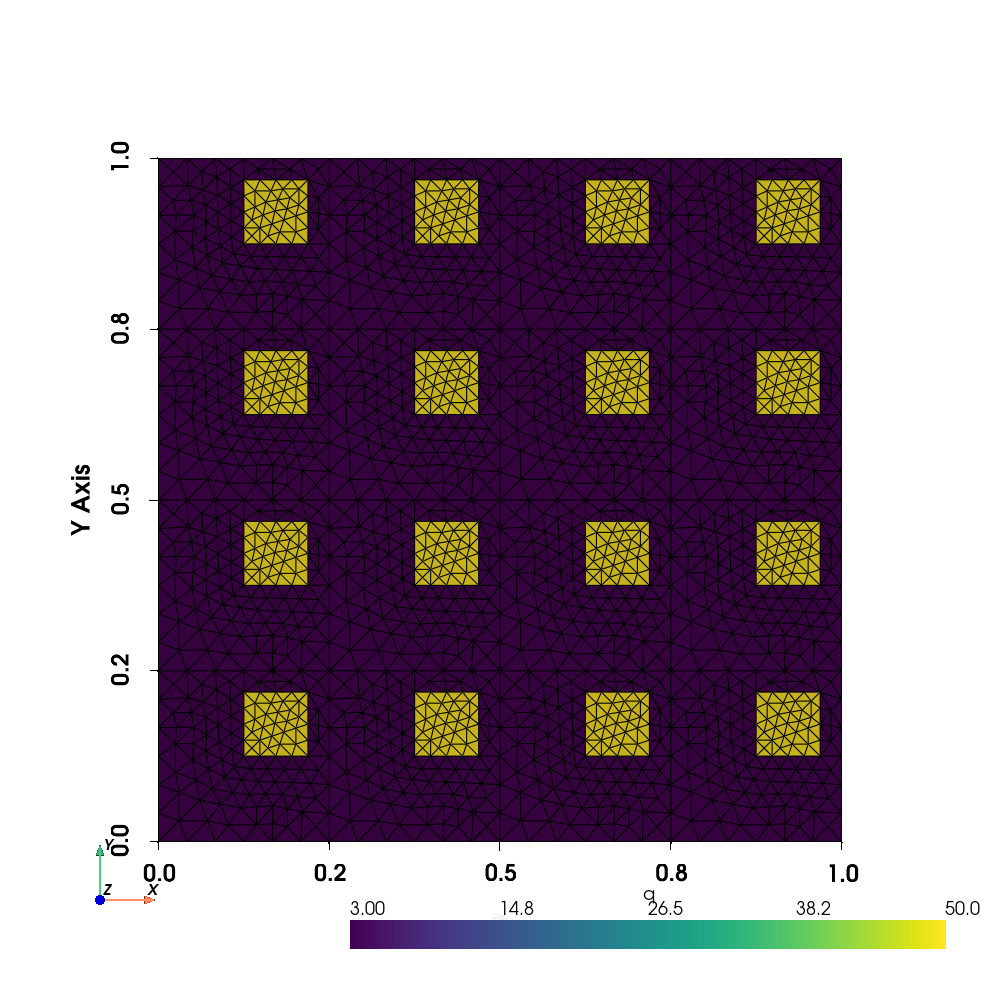
\includegraphics[width=0.85\textwidth]{Figures/q.png}
  \caption{Koeficijent toplinske vodljivosti $\kappa$}
  \label{fig:kappa}
\end{figure}

\begin{figure}[h]
  \centering
  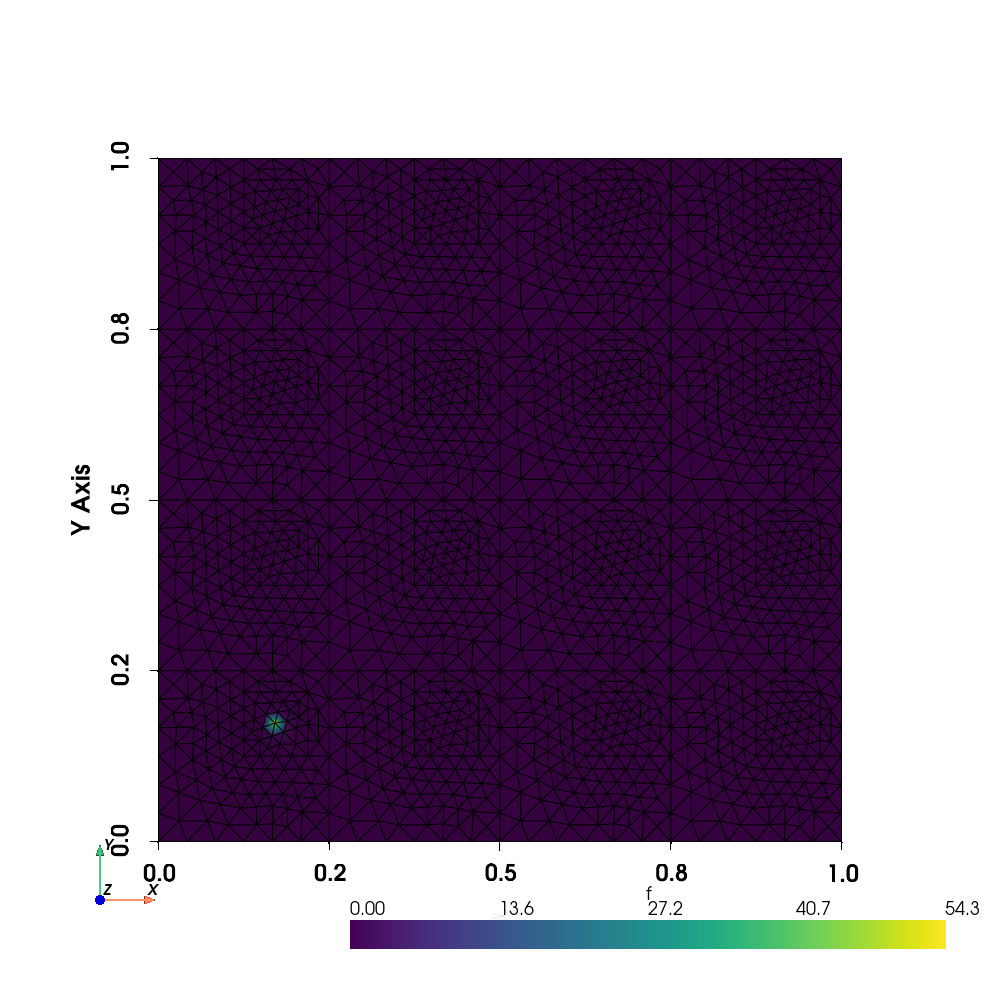
\includegraphics[width=0.85\textwidth]{Figures/f.png}
  \caption{Izvor topline $f$}
  \label{fig:f}
\end{figure}

%-------------------------------------------------------------------------------
\chapter{Implementacija}

\section{Biblioteka FEniCSx/dolfinx}

Projekt FEniCS istraživački je i softverski projekt usmjeren na stvaranje matematičkih metoda
i softvera za rješavanje parcijalnih diferencijalnih jednadžbi.
Projekt je \textit{open-source}, započet 2003.\ godine i razvija se u suradnji istraživača s brojnih sveučilišta
i istraživačkih instituta diljem svijeta. Najnovija verzija FEniCS projekta, FEniCSx,
sastoji se od nekoliko osnovnih elemenata: DOLFINx, UFL, FFCx i Basix.

DOLFINx je visoko učinkoviti C++ sustav FEniCSx-a,
gdje su implementirane strukture poput mreža, funkcijskih prostora i funkcija.
Osim toga, DOLFINx također sadrži računski intenzivne funkcije kao što su sastavljanje konačnih elemenata
i algoritmi za rafiniranje mreže. Također pruža sučelje za rješavače linearne algebre i podatkovne strukture, kao što je PETSc.

UFL je jezik visokog nivoa za opisivanje varijacijskih formulacija s matematičkom sintaksom visokog nivoa.

FFCx jezični je procesor formi za FEniCSx, odnosno, s obzirom na varijacijske formulacije napisane s UFL-om,
generira učinkovit kod u programskom jeziku C.

Basix je sustav za konačne elemente FEniCSx-a, odgovoran za generiranje baza funkcija konačnih elemenata.

Kao što smo već spomenuli, mi ćemo koristiti Python sučelje za FEniCSx, odnosno DOLFINx, kako bismo implementirali našu metodu.


\section{Algoritam}

Prikazat ćemo glavni dio izvornog koda, koji smo opisali u glavnom dijelu rada.
Korake koje je potrebno obaviti prije samo ćemo iskomentirati.

\renewcommand\thechapter{\arabic{chapter}}

\begin{lstlisting}[
  language={Python},
  label={lst:multiscale_main},
  caption={Glavni dio}
]
# Create coarse mesh msh_c and load its cell tags ct_c and facet tags ft_c
# By refining msh_c, create fine mesh msh_f and read/transfer its cell tags ct_f and facet tags ft_f
# Create parent_cells array, where parent_cells[t] is the index of the parent cell of fine cell t
# Create function spaces FS_c and FS_f on msh_c and msh_f respectively
# Create coefficient function kappa and right-hand-side source function f on FS_f

num_dofs_c = FS_c.dofmap.index_map.size_local * FS_c.dofmap.index_map_bs  # N_H
num_dofs_f = FS_f.dofmap.index_map.size_local * FS_f.dofmap.index_map_bs  # N_h

# Define Dirichlet boundary condition on fine mesh
boundary_facets_f = ft_f.find(dc_boundary_marker)  # dc_boundary_marker is some boundary marker for Dirichlet boundary
boundary_dofs_f = fem.locate_dofs_topological(FS_f, msh_f.topology.dim - 1, boundary_facets_f)
bcs_f = [fem.dirichletbc(dolfinx.default_scalar_type(0), boundary_dofs_f, FS_f)]

# Create boundary correction (restriction) matrix B_H
boundary_facets_c = ft_c.find(dc_boundary_marker)
boundary_dofs_c = fem.locate_dofs_topological(FS_c, 1, boundary_facets_c)
not_boundary_dofs_c = np.setdiff1d(np.arange(num_dofs_c), boundary_dofs_c, assume_unique=True)
B_H = csr_matrix(
    (
        np.ones_like(not_boundary_dofs_c),
        (
            not_boundary_dofs_c,
            not_boundary_dofs_c
        )
    ),
    shape=(num_dofs_c, num_dofs_c)
)
assert B_H.shape == (num_dofs_c, num_dofs_c)

# Remove all-zero rows from B_H
B_H = csr_matrix((B_H.data, B_H.indices, np.unique(B_H.indptr)), shape=(len(ind_ptr) - 1, B_H.shape[1]))

# Define our problem on fine mesh using UFL
# and assemble the fine stiffness matrix A_h
# and fine mass matrix M_h
u_f = TrialFunction(FS_f)
v_f = TestFunction(FS_f)
a = inner(kappa * grad(u_f), grad(v_f)) * dx
m = inner(u_f, v_f) * dx
L = inner(f, v_f) * dx

fine_stiffness_assembler = LocalAssembler(a)

A_h = assemble_matrix(form(a), bcs_f).to_scipy()
M_h = assemble_matrix(form(m), bcs_f).to_scipy()
f_h = assemble_vector(form(L)).array

# Create projection matrix P_h from coarse mesh Lagrange space to fine mesh Lagrange space
P_h = csr_matrix(interpolation_matrix_non_matching_meshes(FS_f, FS_c).transpose())

# Calculate constraint matrix C_h
C_h = P_h @ M_h

# Create corrector matrix Q_h
Q_h = compute_correction_operator(msh_c, ct_c, parent_cells,
                                  FS_c, FS_f,
                                  boundary_dofs_c, boundary_dofs_f,
                                  A_h, P_h, C_h,
                                  fine_stiffness_assembler)

# Add the corrector matrix to the solution and solve the system
A_H_LOD = B_H @ (P_h + Q_h) @ A_h @ (P_h + Q_h).transpose() @ B_H.transpose()
f_H = B_H @ (P_h + Q_h) @ f_h
u_H_LOD = B_H.transpose() @ spsolve(A_H_LOD, f_H_LOD)
u_h_LOD = (P_h + Q_h).transpose() @ u_H_LOD

# u_h_LOD is now a vector of size num_dofs_f, which we can wrap in a Function object using dolfinx
# and display using pyvista or ParaView
uhLOD = Function(FS_f)
uhLOD.x.array.real = u_h_LOD
# ...
\end{lstlisting}


\begin{lstlisting}[
  language={Python},
  label={lst:multiscale_compute_correction_operator},
  caption={Funkcija za računanje operatora korekcije}
]
def compute_correction_operator(
    msh_c: mesh.Mesh,
    ct_c: mesh.MeshTags,
    parent_cells: np.ndarray,
    FS_c: fem.FunctionSpaceBase,
    FS_f: fem.FunctionSpaceBase,
    coarse_boundary_dofs: np.ndarray,
    fine_boundary_dofs: np.ndarray,
    A_h: csr_matrix,
    P_h: csr_matrix,
    C_h: csr_matrix,
    fine_stiffness_assembler: LocalAssembler,
) -> lil_matrix:

    num_dofs_c = FS_c.dofmap.index_map.size_local * FS_c.dofmap.index_map_bs  # N_H
    num_dofs_f = FS_f.dofmap.index_map.size_local * FS_f.dofmap.index_map_bs  # N_h

    Q_h = lil_matrix((num_dofs_c, num_dofs_f))

    # For each coarse cell K_l
    for l in ct_c.indices:
        # Create local patch U_l consisting of K_l with one layer of neighboring cells (k = 1, for now)
        incident_facets = mesh.compute_incident_entities(msh_c.topology, l, 2, 1)
        incident_vertices = mesh.compute_incident_entities(msh_c.topology, l, 2, 0)
        coarse_patch_1 = mesh.compute_incident_entities(
            msh_c.topology, incident_facets, 1, 2
        )
        coarse_patch_2 = mesh.compute_incident_entities(
            msh_c.topology, incident_vertices, 0, 2
        )
        coarse_patch = np.unique(np.concatenate((coarse_patch_1, coarse_patch_2)))

        # Find coarse dofs on patch
        coarse_dofs_local = fem.locate_dofs_topological(
            FS_c, 2, coarse_patch
        )  # Z_l[i] = coarse_dofs_local[i]
        coarse_dofs_local = np.setdiff1d(
            coarse_dofs_local, coarse_boundary_dofs, assume_unique=True
        )
        num_coarse_dofs_local = coarse_dofs_local.size  # N_H_l

        # Create restriction matrix R_H_l (N_H_l x N_H)
        R_H_l = csr_matrix(
            (
                np.ones_like(coarse_dofs_local),
                (np.arange(num_coarse_dofs_local), coarse_dofs_local),
            ),
            shape=(num_coarse_dofs_local, num_dofs_c),
        )

        # Find fine cells on patch
        fine_patch = np.where(np.isin(parent_cells, coarse_patch))[0]

        # Find fine dofs on patch
        fine_dofs_local = fem.locate_dofs_topological(
            FS_f, 2, fine_patch
        )  # z_l[i] = fine_dofs_local[i]
        fine_dofs_local = np.setdiff1d(
            fine_dofs_local, fine_boundary_dofs, assume_unique=True
        )
        num_fine_dofs_local = fine_dofs_local.size  # N_h_l

        # Create restriction matrix R_h_l (N_h_l x N_h)
        R_h_l = csr_matrix(
            (
                np.ones_like(fine_dofs_local),
                (np.arange(num_fine_dofs_local), fine_dofs_local),
            ),
            shape=(num_fine_dofs_local, num_dofs_f),
        )
        assert R_h_l.shape == (num_fine_dofs_local, num_dofs_f)

        # Create local coarse-node-to-coarse-element restriction matrix T_H_l (c_d x N_H)
        l_global_dofs = fem.locate_dofs_topological(FS_c, 2, l)  # p[i] = l_dofs[i]
        assert l_global_dofs.size == msh_c.topology.cell_types[0].value
        T_H_l = csr_matrix(
            (
                np.ones_like(l_global_dofs),
                (np.arange(l_global_dofs.size), l_global_dofs),
            ),
            shape=(l_global_dofs.size, num_dofs_c),
        )
        assert T_H_l.shape == (l_global_dofs.size, num_dofs_c)

        # Calculate local stiffness matrix and constraints matrix
        A_l = R_h_l @ A_h @ R_h_l.transpose()
        C_l = R_H_l @ C_h @ R_h_l.transpose()

        # In order to create local load vector matrix,
        # we need the contributions of local stiffness matrices on fine cells
        sigma_A_sigmaT_l = lil_matrix((num_dofs_f, num_dofs_f))
        # Find fine cells only on coarse cell l
        fine_cells_on_l = np.where(parent_cells == l)[0]
        for t in fine_cells_on_l:
            # Assemble local stiffness matrix A_t
            A_t = fine_stiffness_assembler.assemble_matrix(t)
            A_t = csr_matrix(A_t)

            # Find global fine dofs on fine cell t
            fine_dofs_global_t = fem.locate_dofs_topological(FS_f, 2, t)
            # Create local-to-global-mapping sigma_t
            sigma_t = csr_matrix(
                (
                    np.ones_like(fine_dofs_global_t),
                    (np.arange(fine_dofs_global_t.size), fine_dofs_global_t),
                ),
                shape=(fine_dofs_global_t.size, num_dofs_f),
            )

            # Add the contribution
            sigma_A_sigmaT_l += sigma_t.transpose() @ A_t @ sigma_t

        # Create local load vector matrix
        r_l = -(T_H_l @ P_h @ sigma_A_sigmaT_l @ R_h_l.transpose())

        # Compute the inverse of the local stiffness matrix
        A_l_inv = csr_matrix(inv(A_l.todense()))

        # Precomputations related to the operator
        Y_l = A_l_inv @ C_l.transpose()

        # Compute inverse Schur complement
        S_l_inv = csr_matrix(inv((C_l @ Y_l).todense()))

        # Compute correction for each coarse space function with support on K_l
        w_l = lil_matrix((l_global_dofs.size, num_fine_dofs_local))
        for i in range(l_global_dofs.size):
            q_i = A_l_inv @ r_l[i].transpose()
            lambda_i = S_l_inv @ (C_l @ q_i)
            w_l_i = q_i - Y_l @ lambda_i
            w_l[i] = w_l_i.transpose()

        # Update the corrector matrix
        Q_h += T_H_l.transpose() @ w_l @ R_h_l

    return Q_h
\end{lstlisting}

\renewcommand\thechapter{\arabic{chapter}.}

%-------------------------------------------------------------------------------
\chapter{Rezultati i rasprava}
\label{pog:rezultati_i_rasprava}

Na slici\ \ref{fig:sol_fine} prikazano je "točno" rješenje, odnosno rješenje koje dobijemo
ugrubim rješavanjem problema na finoj skali.
Na slici\ \ref{fig:sol_coarse} prikazano je rješenje dobiveno grubim rješavanjem problema na gruboj skali,
dakle bez uvođenja korekcije.

\begin{figure}[h]
  \centering
  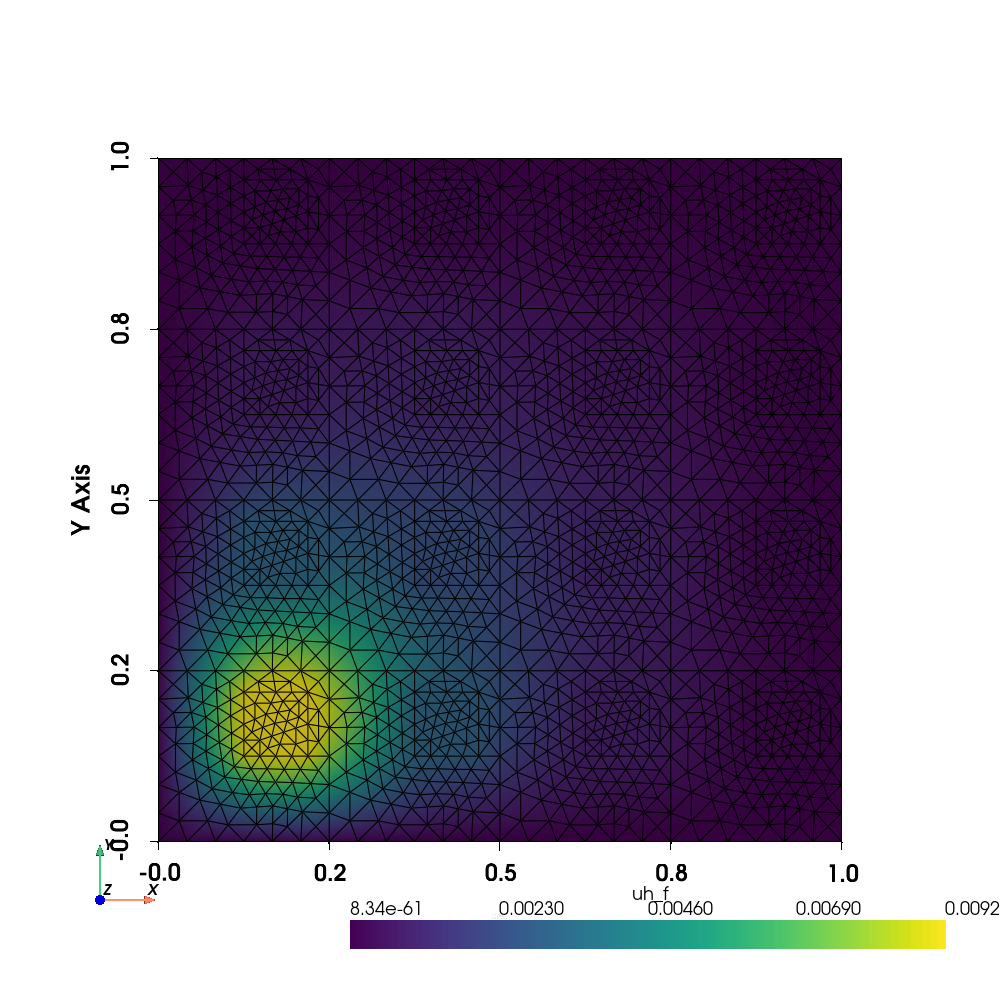
\includegraphics[width=0.85\textwidth]{Figures/solution_fine.png}
  \caption{Rješenje na finoj skali}
  \label{fig:sol_fine}
\end{figure}

\begin{figure}[h]
  \centering
  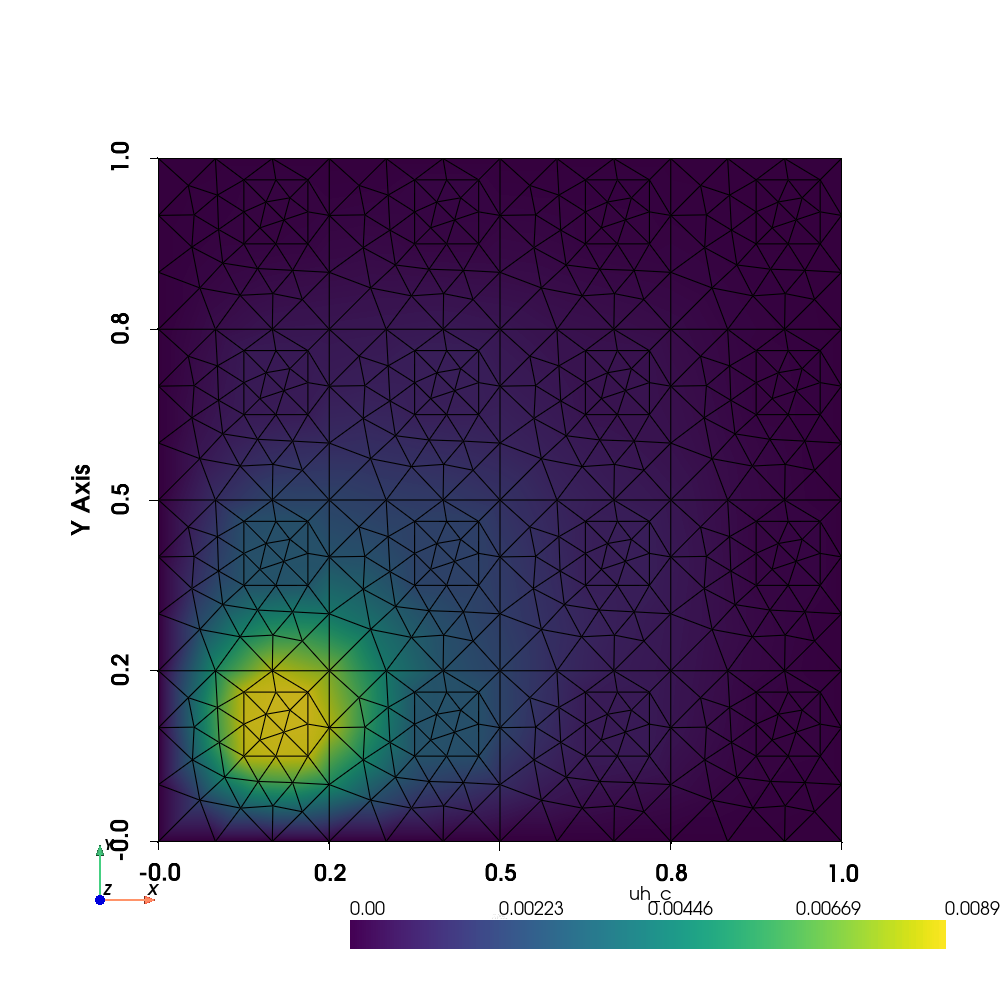
\includegraphics[width=0.85\textwidth]{Figures/solution_coarse.png}
  \caption{Rješenje na gruboj skali}
  \label{fig:sol_coarse}
\end{figure}

Na slici\ \ref{fig:sol_lod} prikazano je rješenje dobiveno uvođenjem korekcije,
odnosno korištenjem opisane metode. Onako od oka, a i na slici slici\ \ref{fig:sol_diff},
možemo primijetiti da je rješenje dobiveno uvođenjem korekcije izuzetno slično finom rješenju.

\begin{figure}[h]
  \centering
  \includegraphics[width=0.85\textwidth]{Figures/solution_lod.png}
  \caption{LOD rješenje}
  \label{fig:sol_lod}
\end{figure}

\begin{figure}[h]
  \centering
  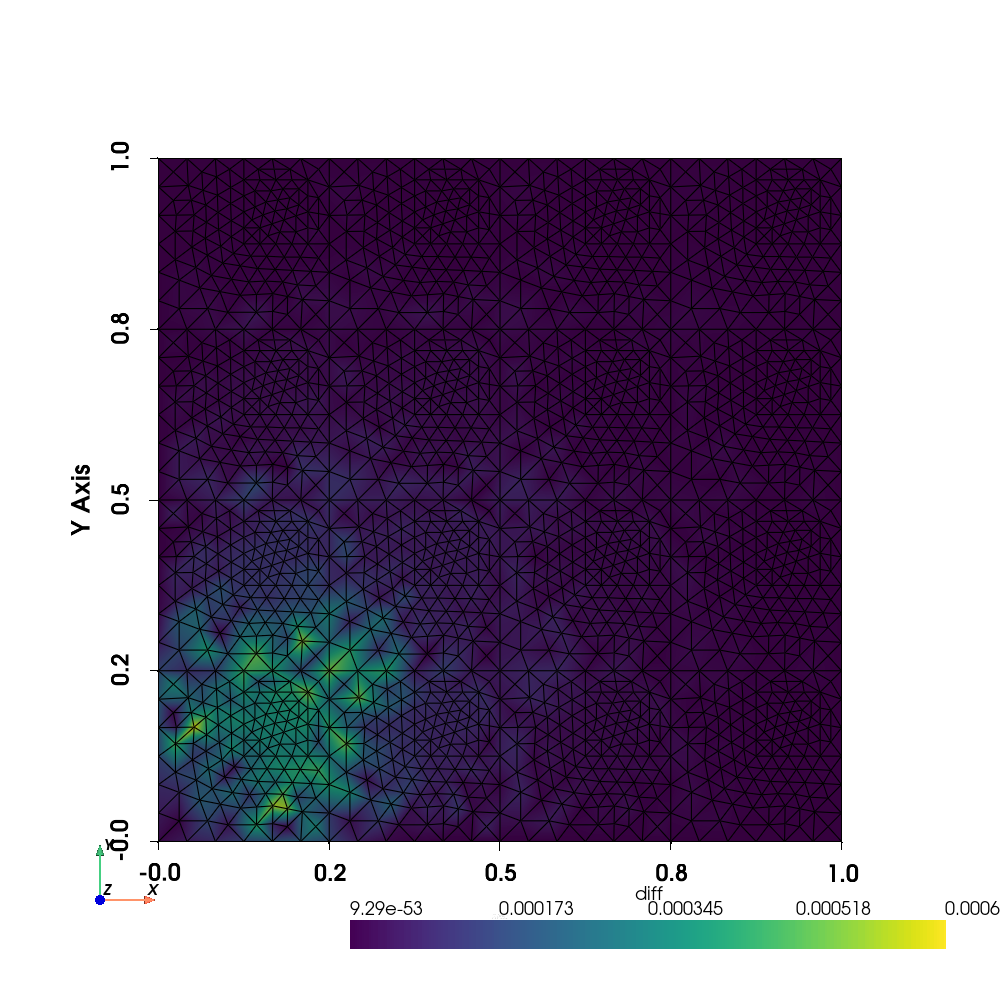
\includegraphics[width=0.85\textwidth]{Figures/solution_diff.png}
  \caption{Razlika između finog rješenja i LOD rješenja}
  \label{fig:sol_diff}
\end{figure}

Na grafu\ \ref{fig:diag_comp}, koji prikazuje vrijednosti rješenja na dijagonali domene,
tu usporedbu možemo bolje vidjeti. Dakle, čak i pri maksimalnom odstupanju,
ono iznosi tek 5–7\% maksimalne vrijednosti funkcija.

\begin{figure}[h]
  \centering
  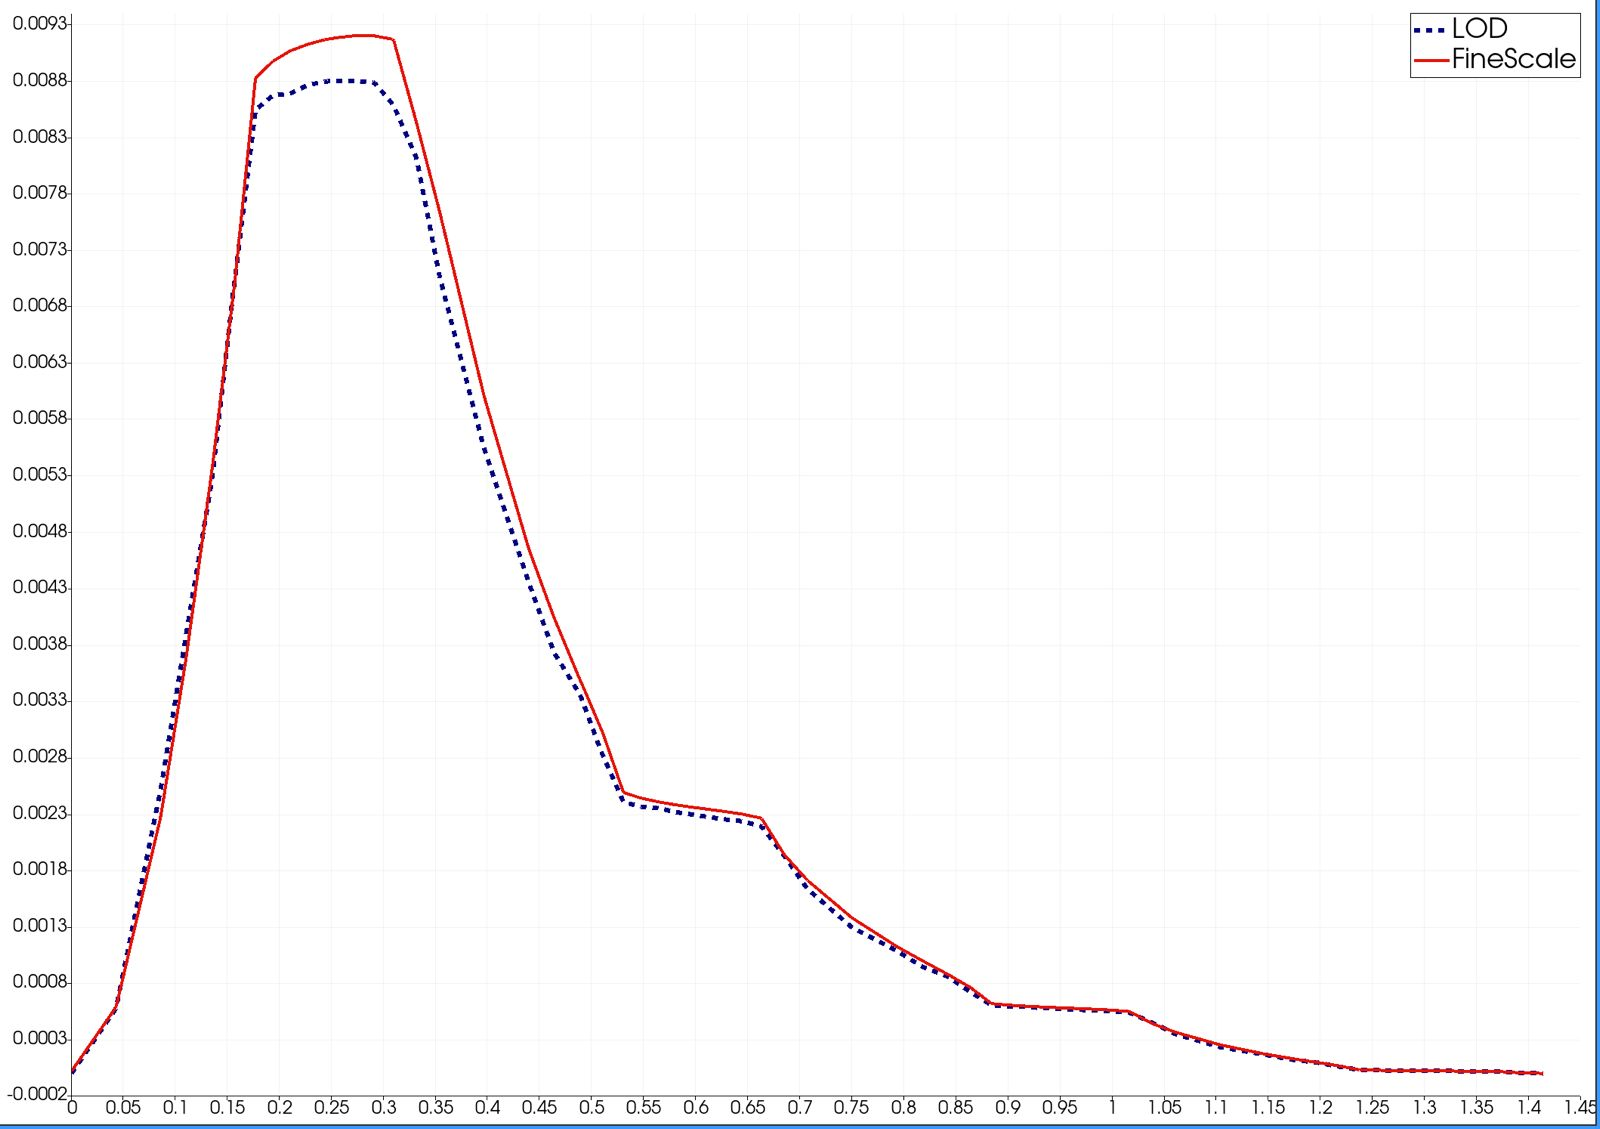
\includegraphics[width=0.85\textwidth]{Figures/diag_diff.jpg}
  \caption{Usporedba finog rješenja i LOD rješenja na dijagonali domene}
  \label{fig:diag_comp}
\end{figure}

Dakle, sada možemo biti prilično optimistični da rješenje daje prihvatljivo precizne odnosno točne rezultate.
Međutim, izmjerimo li vrijeme potrebno za izračun rješenja ovog primjera, vidimo da izračun operatora korekcije
uzima nekoliko desetaka sekundi, dok ugrubo rješavanje problema na finoj skali traje manje od sekunde.
Objašnjenje leži u tome da se radi o vrlo jednostavnom primjeru, s brojem stupnjeva slobode mesha mjerljivim u tisućama,
što je i dalje jako jednostavan problem računalu za riješiti grubom silom. Također, prave prednosti ove metode nismo se još
ni dotaknuli, a to je mogućnost paralelizacije izračuna operatora korekcije, budući da doprinos
svake pojedine ćelije možemo računati paralelno.

Stoga, u budućem radu planiramo implementirati paralelizaciju izračuna operatora korekcije,
kao i ostale moguće optimizacije i poboljšanja (primjerice uvođenje više slojeva susjednih ćelija u lokalnu zakrpu,
korištenje informacije da je većina lokalnih matrica krutosti rijetka za efikasnije računanje njihovih inverza,
uvođenje više slojeva korekcije, itd.). Također, planiramo primijeniti metodu na mnogo složenijim primjerima i
s mnogo većim brojem stupnjeva slobode na finoj skali.



%--- ZAKLJUČAK / CONCLUSION ----------------------------------------------------
\chapter{Zaključak}
\label{pog:zakljucak}

Predstavili smo metodu lokalizirane ortogonalne dekompozicije, jednu od višeskalnih metoda konačnih elemenata
korištenih za rješavanje raznih fizikalnih problema s parcijalnim diferencijalnim jednadžbama. Metoda se temelji na efikasnom rješavanju problema na gruboj skali,
kako bi se dobila aproksimacija rješenja, a zatim se uvođenjem operatora korekcije hvaćaju mikroskopska svojstva materijala fine skale.
Detaljno smo opisali teorijsku podlogu iza metode kao i korake potrebne za njezinu implementaciju.
Implementirali smo metodu u programskom jeziku Python koristeći biblioteku FEniCSx/dolfinx
i prikazali smo rezultate na jednostavnom primjeru širenja topline. Rezultati su pokazali da metoda daje točne rezultate,
no u budućem radu potrebno je pokazati kako je iste rezultate na dovoljno velikim i inače zahtjevnim primjerima
moguće dobiti uz značajno manje računalne resurse nego što bi to bilo potrebno rješavanjem problema ugrubo na finoj skali.
U budućem radu ćemo također implementirati i paralelizaciju izračuna operatora korekcije, kao i brojne ostale moguće optimizacije i poboljšanja,
te na kraju primijeniti metodu na mnogo složenijim primjerima i s mnogo većim brojem stupnjeva slobode na finoj skali.
Očekujemo da će metoda pokazati svoju pravu snagu upravo na takvim primjerima, na samo što se tiče vremenskog troška izvođenja,
već i konvergencije greške u ovisnosti o mjeri gustoće mreže.

%--- LITERATURA / REFERENCES ---------------------------------------------------

% Literatura se automatski generira iz zadane .bib datoteke / References are automatically generated from the supplied .bib file
% Upiši ime BibTeX datoteke bez .bib nastavka / Enter the name of the BibTeX file without .bib extension
\bibliography{literatura}



%--- SAŽETAK / ABSTRACT --------------------------------------------------------

% Sažetak na hrvatskom
\begin{sazetak}
  U ovom radu iznijeli smo teorijsku podlogu iza metoda konačnih elemenata za rješavanje diferencijalnih jednadžbi
  i objasnili potrebu za uvođenjem višeskalnih metoda, do koje često dolazi zbog mikroskopskih visoko-oscilirajućih svojstava
  heterogenih kompozitnih materijala. Detaljno smo opisali metodu lokalizirane ortogonalne dekompozicije,
  koja se temelji na ortogonalnoj podjeli prostora rješenja na grubu skalu, na kojoj se ono može efikasno izračunati,
  i finu skalu, kojom ciljamo uhvatiti mikroskopska svojstva materijala. Implementirali smo metodu u programskom jeziku Python,
  koristeći biblioteku FEniCSx/dolfinx, te prikazali rezultate na jednostavnom primjeru širenja topline, odnosno Poissonove jednadžbe.
\end{sazetak}

\begin{kljucnerijeci}
  \frenchspacing
  Metode konačnih elemenata; FEM; Višeskalne metode; MsFEM; Lokalizirana ortogonalna dekompozicija; LOD;
  FEniCSx; dolfinx; Poissonova jednadžba; Širenje topline; Heterogeni materijali; Kompozitni materijali
  \nonfrenchspacing
\end{kljucnerijeci}


% Abstract in English
\begin{abstract}
  In this paper, we presented the theoretical background behind finite element methods for solving differential equations
  and explained the need for introducing multiscale methods, which often arises due to the microscopic highly oscillatory properties
  of heterogeneous composite materials. We explained in detail the localized orthogonal decomposition method,
  which is based on an orthogonal decomposition of the solution space into a coarse scale, where the solution can be efficiently computed,
  and a fine scale, which aims to capture the microscopic properties of the material. We implemented the method in Python,
  using the FEniCSx/dolfinx library, and presented the results on a simple example of heat conduction, i.e.\ the Poisson equation.
\end{abstract}

\begin{keywords}
  \frenchspacing
  Finite element method; FEM; Multiscale methods; MsFEM; Localized orthogonal decomposition; LOD;
  FEniCSx; dolfinx; Poisson equation; Heat conduction; Heterogeneous materials; Composite materials
  \nonfrenchspacing
\end{keywords}


%--- PRIVITCI / APPENDIX -------------------------------------------------------

% Sva poglavlja koja slijede će biti označena slovom i riječi privitak / All following chapters will be denoted with an appendix and a letter
\backmatter

%\chapter{Izvorni kod}

% \lstinputlisting[language=Python]{src/multiscale.py}


\end{document}
